\documentclass[10pt,a4paper]{article}
\usepackage[margin=18mm]{geometry}
\usepackage[T1]{fontenc}
\usepackage{lmodern,graphicx,booktabs,amsmath,amssymb,xcolor}
\usepackage[hidelinks]{hyperref}
\setlength{\parindent}{0pt}
\setlength{\parskip}{6pt}
\begin{document}
{\Large\bfseries Actual C7 three-torsion divisors and integral basis}\par
23 November 2026 \quad Native correctness; unsigned [pcc:unverified]

\textbf{Outcome.} The complete fixed geometric three-torsion cohort
supports sign $-1$: all eight nonzero points have conic
principal-divisor certificates. Sign $+1$ has common-divisor degree zero
in every cell. The resulting written descent constructs the divided
map and an integral H basis using the actual curve correspondences.

\begin{center}
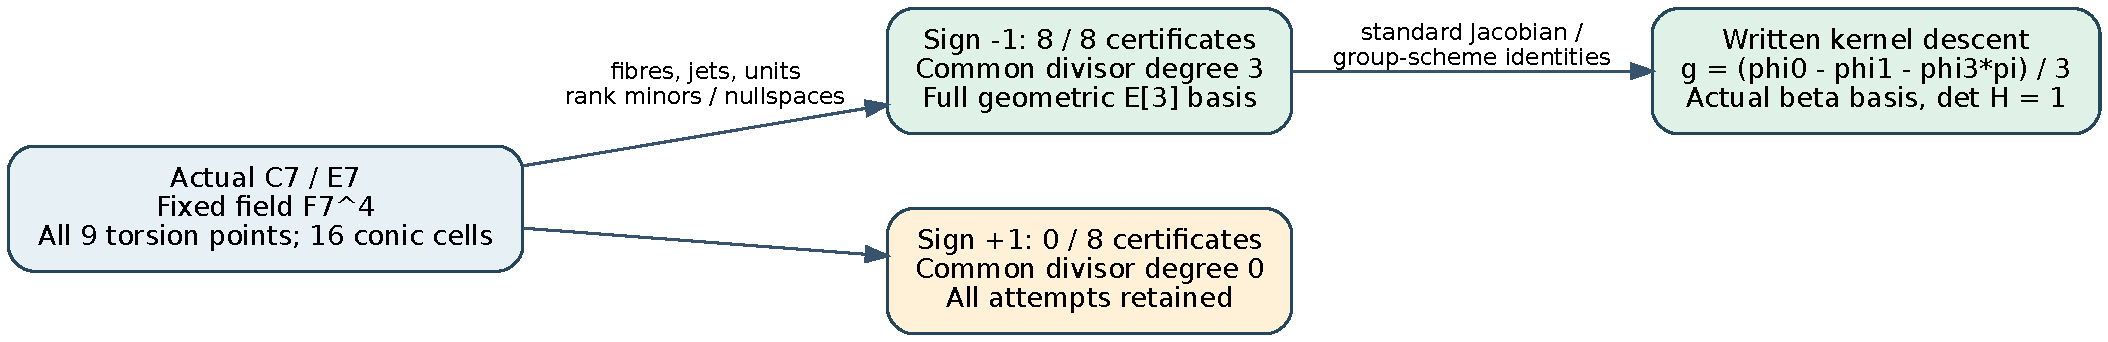
\includegraphics[width=\linewidth,height=57mm,keepaspectratio]{certificate.pdf}
\end{center}

\textbf{Full cohort, with multiplicities.} Work over
$K=\mathbb F_7[a]/(a^4+5a^2+5)$, encoding elements by their base-seven
coefficient integer. Scan all 2401 field elements against the actual
division polynomial $3x^4+5x^2+2x+3$ for
$E:y^2=x^3+2x+6$. Retain all nine points, including $O$.
For every nonzero point and both signs impose the complete divisor
conditions
\[
 D_s(P)=f_0^{-1}(P)+f_3^{-1}(s\pi P)-f_1^{-1}(P)-3P_-,
 \qquad P_-=[1:0:-1].
\]
The degree-two/three fibre algebras and third-order curve jet impose five
conditions on each conic. All positive and negative constraint ranks are
five. All four opposite-divisor unit tests pass in every cell.

\begin{center}
\begin{tabular}{lrr}
\toprule
Actual point $(x,y)$ in the fixed encoding & Common degree $s=+1$ & $s=-1$\\
\midrule
$(54,7)$ &0&3\\
$(54,42)$ &0&3\\
$(104,343)$ &0&3\\
$(104,2058)$ &0&3\\
$(248,1050)$ &0&3\\
$(248,1400)$ &0&3\\
$(294,364)$ &0&3\\
$(294,2086)$ &0&3\\
\bottomrule
\end{tabular}
\end{center}

\textbf{Exact divisor certificate.} Coprime conics have a length-four
complete intersection; all sixteen coprimality ranks are six. Its
degree-two and degree-six spaces have dimension four by the Koszul
resolution. Adjoining the actual quartic gives a $36\times28$ degree-six
Macaulay matrix. Rank 25 gives common degree three for sign $-1$;
rank 28 gives degree zero for sign $+1$. Nonzero original-row minors
and full nullspace checks certify these ranks. Opposite units keep the
common divisor away from both prescribed degree-five divisors, so
the degree-three residuals coincide and
$\operatorname{div}_C(q_+/q_-)=D_{-1}(P)$.

All sixteen cells, conics, rank certificates and decisions are retained.
Data d9f917; written proof 05a984.\par
[pcc:unverified]
\newpage
{\Large\bfseries From actual divisors to an integral Jacobian basis}\par

\textbf{A genuine geometric kernel.} Write $\phi_i=f_i^*$ on
$\operatorname{Pic}^0$ and $\pi$ for actual Frobenius. The native
certificates include the full nine-point basis
$P=(54,7)$, $Q=(104,343)$. Thus the actual homomorphism
$h=\phi_0-\phi_1-\phi_3\pi$ kills $E[3]$ geometrically. Since
$\operatorname{char}K=7\ne3$, this kernel is reduced of degree nine.
The standard quotient property of $[3]:E\to E$ supplies the unique
$\mathbb F_7$ homomorphism $g=h/3$.

\textbf{Actual H basis.} The actual $S_3$ curve action gives the cover
Gram $G=\left(\begin{smallmatrix}2&-1&0\\-1&2&0\\0&0&3\end{smallmatrix}\right)$.
Use $\pi^\dagger\pi=7$ and $\pi+\pi^\dagger=-3$. Then
$g^\dagger g=3$, $\phi_1^\dagger g=-1$,
$g^\dagger\phi_3=-\pi^\dagger$, so
\[
 \beta=(\phi_1,-g,g-\phi_3),\quad
 \beta^\dagger\beta=H=
 \begin{pmatrix}2&1&-1\\1&3&\pi\\-1&\pi^\dagger&3\end{pmatrix},
 \quad \det H=1.
\]
The integral left inverse $\alpha=H^{-1}\beta^\dagger$ makes $\beta$
a degree-one isogeny, hence an isomorphism. With $\omega=\pi+2$,
$\omega^2-\omega+5=0$, the actual cover basis is
\[
 B=(\phi_0,\phi_1,\phi_3)=\beta T_-,\qquad
 T_-=\begin{pmatrix}1&1&0\\-(1+\omega)&0&-1\\2-\omega&0&-1\end{pmatrix}.
\]
The preceding zero-of-144 both-sign-compatible mixed-map result remains
valid at its original scope; the actual geometric sign is now supplied
by divisor certificates rather than a preferred catalogue entry.

\textbf{Controls and execution.} All 2401 field Frobenius/inverse checks,
81 group closure and 729 associativity checks pass. Actual conic
coefficient and curve-jet mutations reject and restore; all normalized
conics and cell decisions respect Frobenius. Frozen source
\texttt{5759530} had all 35 complete input/lock readbacks before the
first strict call. All seven phases exit zero with unchanged-input
guards. Rust 1.99.1, warnings denied, overflow/debug assertions,
one worker, 120 seconds / 2 GiB per phase; no source repair.

\textbf{Evidence and scope.} Full stdout is 26469 bytes, SHA256
\texttt{e2beeaae\ldots1279b6a}; all 38 small original files are retained.
The original whole 4735376-byte ELF
\texttt{196720ec\ldots{}d618157} remains in RAM pending approved durable
custody. Standard Jacobian functoriality, quotient descent and the
complete-intersection argument are explicit written dependencies.
This is not a compiled generic Lean theorem or an independent signed
verdict. A separate native certificate audit comes next, then actual
transported S/J4/kernel/pairing/target and divisor evaluation.

\textbf{Sources and continuation.}
\href{https://github.com/isogeny-labs/crypto/tree/575953011ab00e509dd7c25beeaa45e17397c575/research/chained_cm19_3torsion_divisors_20261123}{Frozen source/protocol};
\href{https://github.com/isogeny-labs/crypto/tree/1b04550ed1131174198784468df884807b2d884b/research/chained_cm19_3torsion_divisors_20261123}{complete native result and written proof}.
Quotient and torsion properties: Milne, \emph{Abelian Varieties}, I.7 and I.8, Remark 8.12;
regular-sequence resolution: Stacks, \href{https://stacks.math.columbia.edu/tag/062D}{062D}.
KB/Conductor unavailable; no novelty clearance. Existing custody,
formal, cost-admission and CI requirements persist. [pcc:unverified]
\end{document}
